\chapter{Oracle Aplication Express}

\section{Pengenalan Oracle APEX}
Oracle Aplication Express\cite{OracleApex}. Adalah sebuah wadah dan sarana untuk membuat aplikasi yang menggunakan database Oracle Itu sendiri, dalam akademi oracle ini memajukan ilmu komputer secara global untuk mendorong pengetahuan, inovasi, pengembangan keterampilan, dan keragaman di bidang teknologi. dalam satu tahun terakhir, akademi oracle bekerja dengan lebih dari 15.000 lembaga pendidikan di 128 negara, mendukung lebih dari 6,3 juta siswa di seluruh dunia untuk mempersiapkan mereka untuk berkarir dalam ekonomi global yang digerakkan oleh teknologi.

\section{Tahapan Membuat Aplikasi Oracle Apex}
Pertama kita membuka website https://apex.oracle.com, disini kita akan mendapatkan akses untuk memasuki Oracle Apllication Express, siapkan email anda yang valid untuk membuat Workspace, kita akan langsung mempraktekan bagaimana tahapan pembuatan Aplikasi pada Oracle APEX :

\begin{enumerate}
\item[1] Pergi ke halaman website https://apex.oracle.com/

\begin{figure}[!htbp]
    \begin{center}
    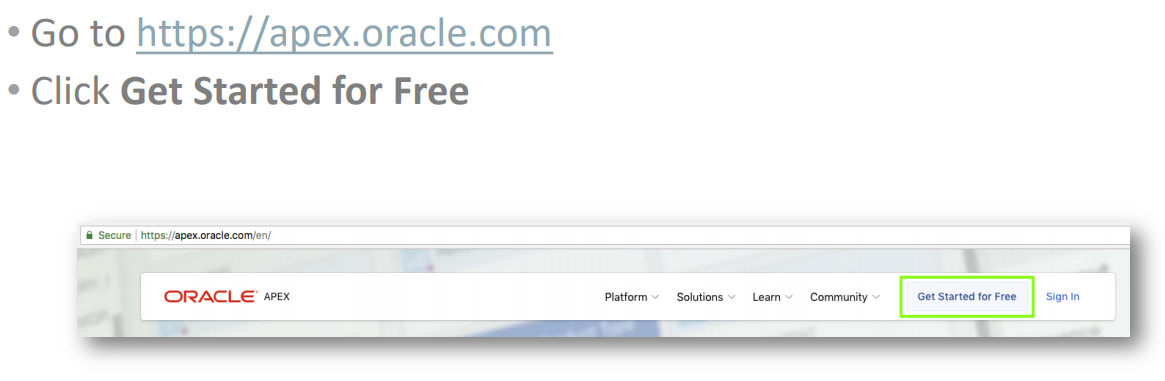
\includegraphics[scale=0.5]{figures/1.PNG}
    \caption{\textit{Get Start For Free.}}
    \end{center}   
    \end{figure}
    
\begin{figure}[!htbp]
\item[2]Klik Request a Free Worksace.

    \begin{center}
    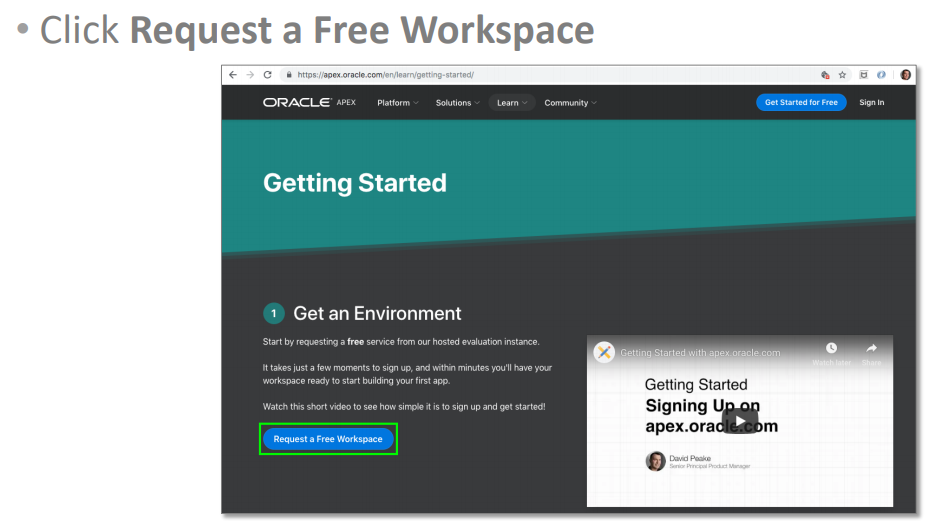
\includegraphics[scale=0.5]{figures/2.PNG}
    \caption{\textit{Request A Free Workspace.}}
    \end{center}

\item[3]Isikan data diri anda seperti nama,email,dan workspace.
        
\item[4]Centang apakah anda pernah melakukan hal tersebut lalu next. 

\item[5]Isikan pada kolom tersebut bebas, mengapa anda ingin menggunakan layanan ini ?, lalu klik next.

\item[6] Centang Accept, lalu klik next.

\item[7] Tahapan terakhir untuk mengkonfirmasi apakah ini anda, lalu klik next.

\label{gambar}
\end{figure}

\begin{figure}
\item[8] Finish, lalu lihat email anda.

    \begin{center}
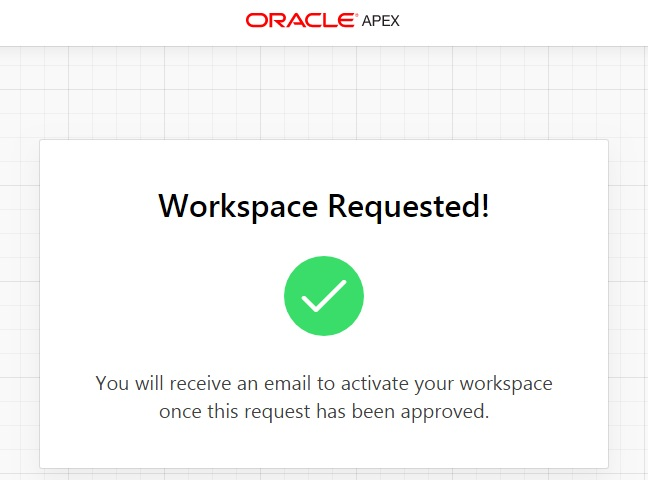
\includegraphics[scale=0.5]{figures/req6.jpg}
    \caption{\textit{Sukses Cek Email.}}
        \end{center}
\label{gambar}
\end{figure}

\begin{figure}
\item[9] Workspace anda telah di Acc lalu klik continue.

    \begin{center}
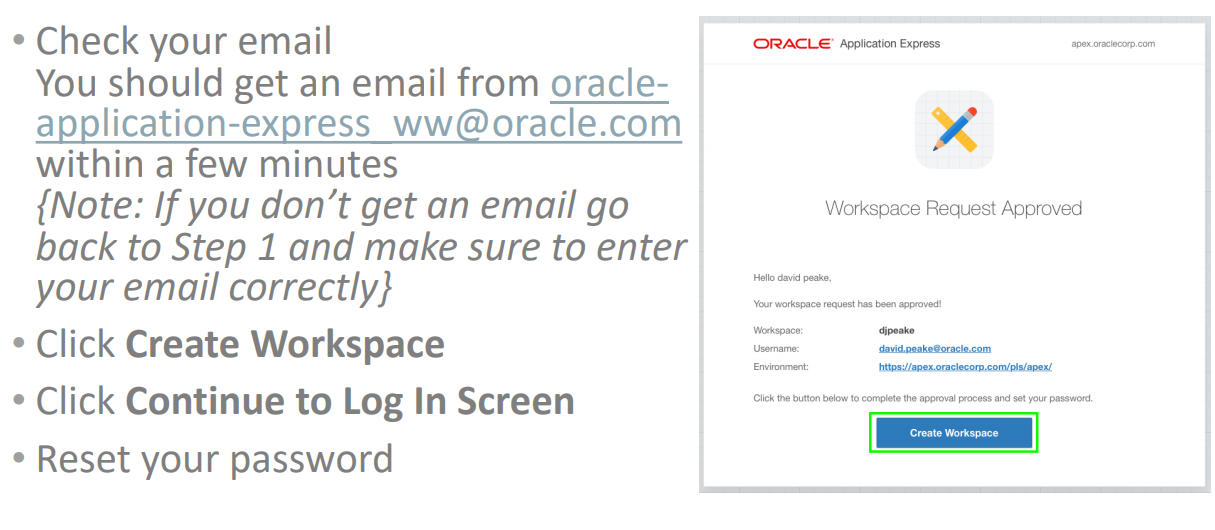
\includegraphics[scale=0.5]{figures/3.PNG}
    \caption{\textit{Email Acc.}}
        \end{center}
\label{gambar}
\end{figure}

\begin{figure}
\item[10] Workspace kamu telah dibut lalu lanjutkan klik sign in.

    \begin{center}
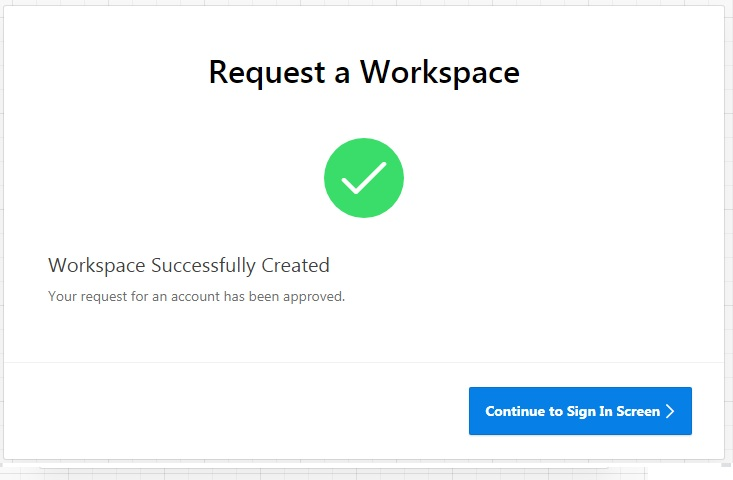
\includegraphics[scale=0.5]{figures/req8.jpg}
    \caption{\textit{Sukses Cek Email.}}
        \end{center}
\label{gambar}
\end{figure}

\begin{figure}
\item[11] Sign in akun anda yang baru saja di buat lalu masuk ke App Builder setelah itu buat App Baru.

    \begin{center}
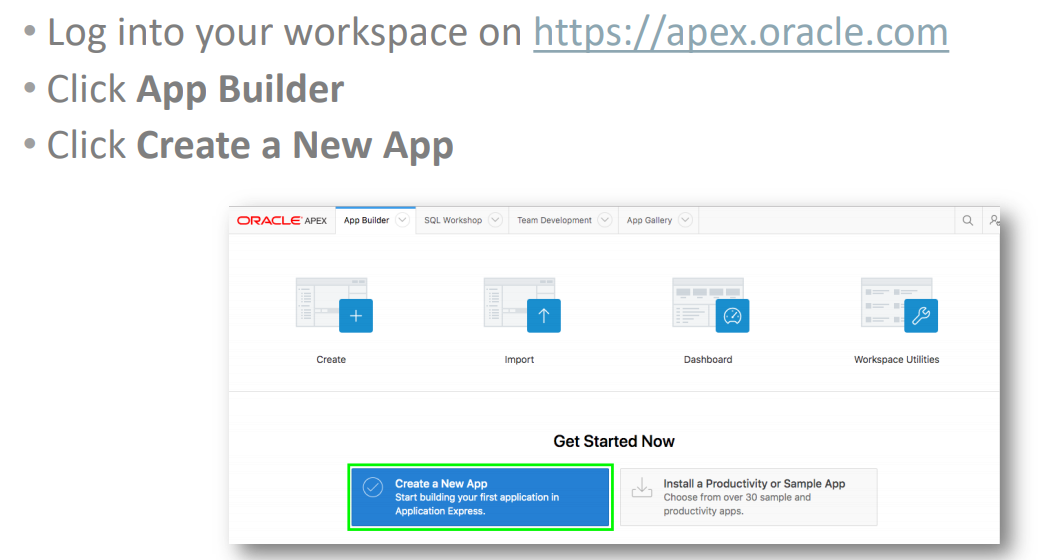
\includegraphics[scale=0.5]{figures/4.PNG}
    \caption{\textit{Logging In.}}
        \end{center}
\label{gambar}
\end{figure}

\begin{figure}
\item[12] Lalu klik dari sebuah file.

    \begin{center}
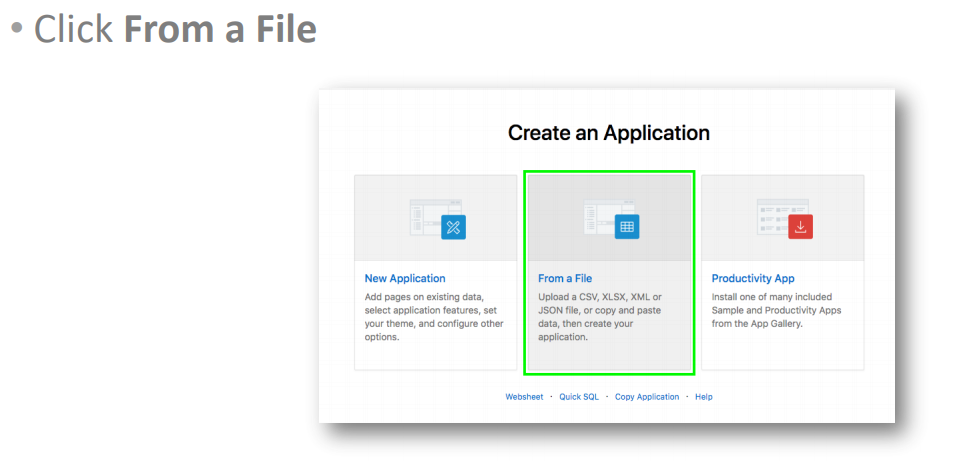
\includegraphics[scale=0.6]{figures/5.PNG}
    \caption{\textit{Selecting App Type.}}
        \end{center}
\label{gambar}
\end{figure}

\begin{figure}
\item[13] Klik Copy dan Paste.

    \begin{center}
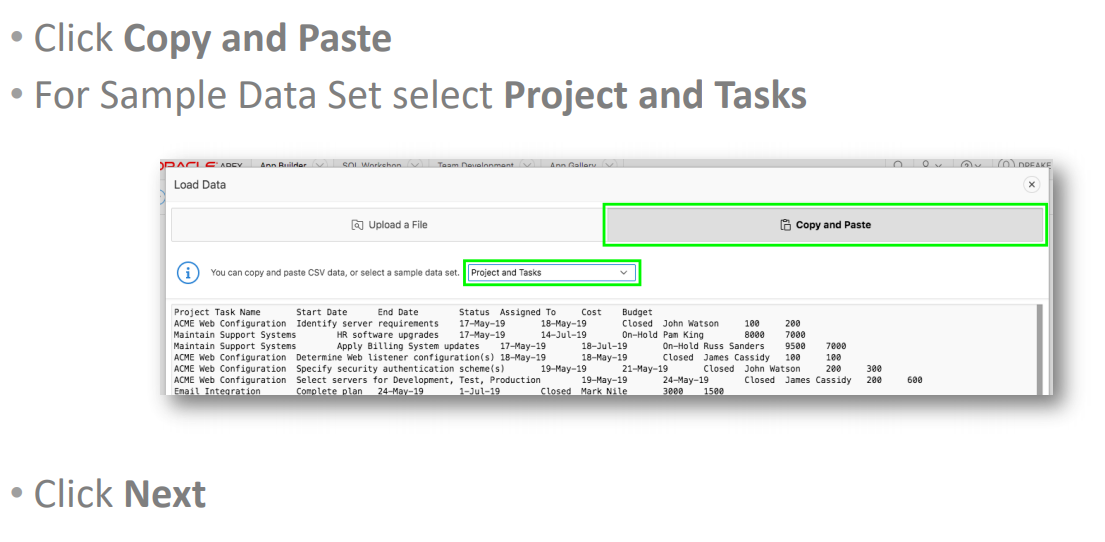
\includegraphics[scale=0.6]{figures/6.PNG}
    \caption{\textit{Loading Sample Data.}}
        \end{center}
\label{gambar}
\end{figure}

\begin{figure}
\item[14] Masuk ke table name dan memuat data.

    \begin{center}
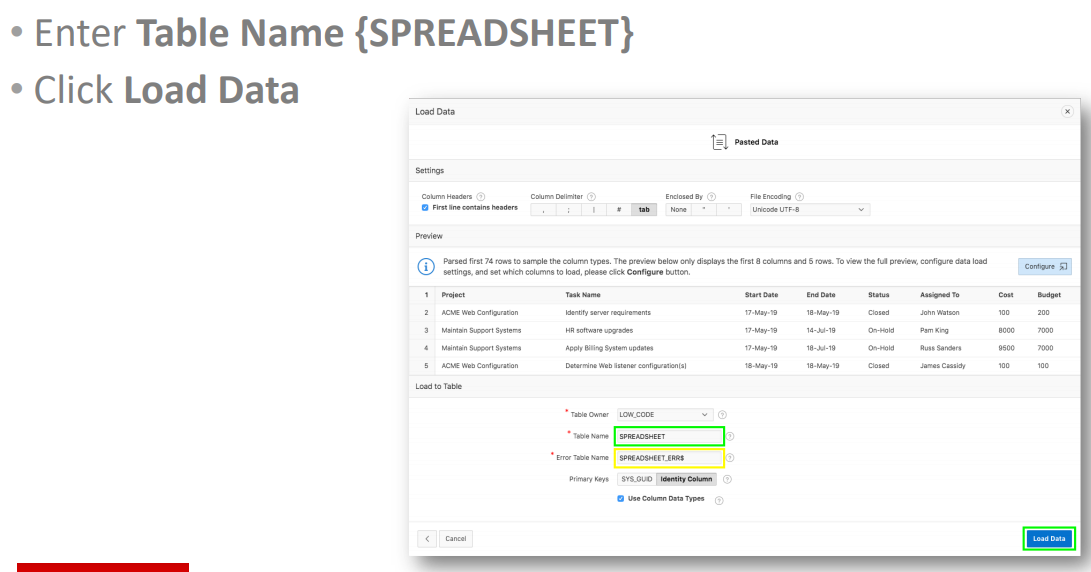
\includegraphics[scale=0.4]{figures/7.PNG}
    \caption{\textit{Naming the Table.}}
        \end{center}
\label{gambar}
\end{figure}

\begin{figure}
\item[15] Setelah Sudah memuat data, tampilan selanjutnya akan seperti berikut.

    \begin{center}
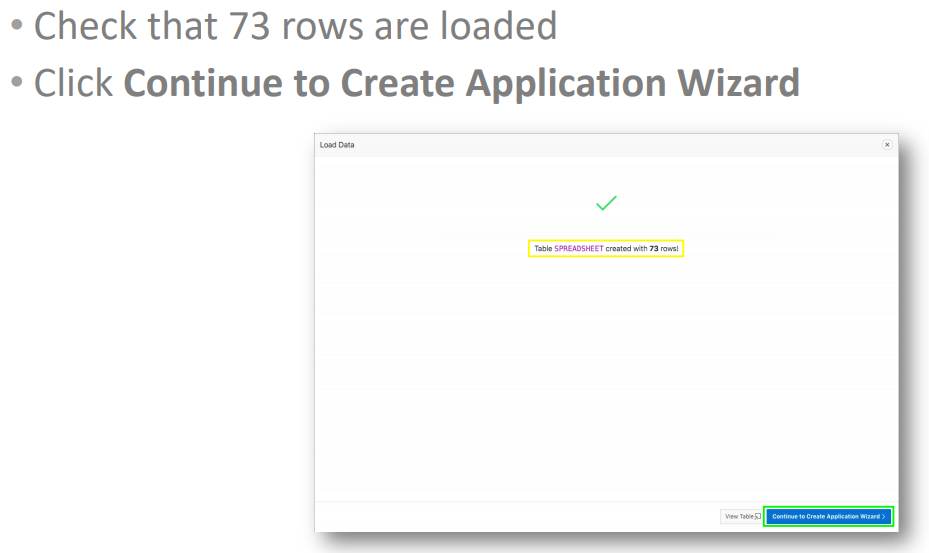
\includegraphics[scale=0.5]{figures/8.PNG}
    \caption{\textit{Verifying Records Loaded}}
        \end{center}
\label{gambar}
\end{figure}

\begin{figure}
\item[16] Lalu Masukan nama, selanjutnya Di sebelah Fitur klik Periksa Semua.

    \begin{center}
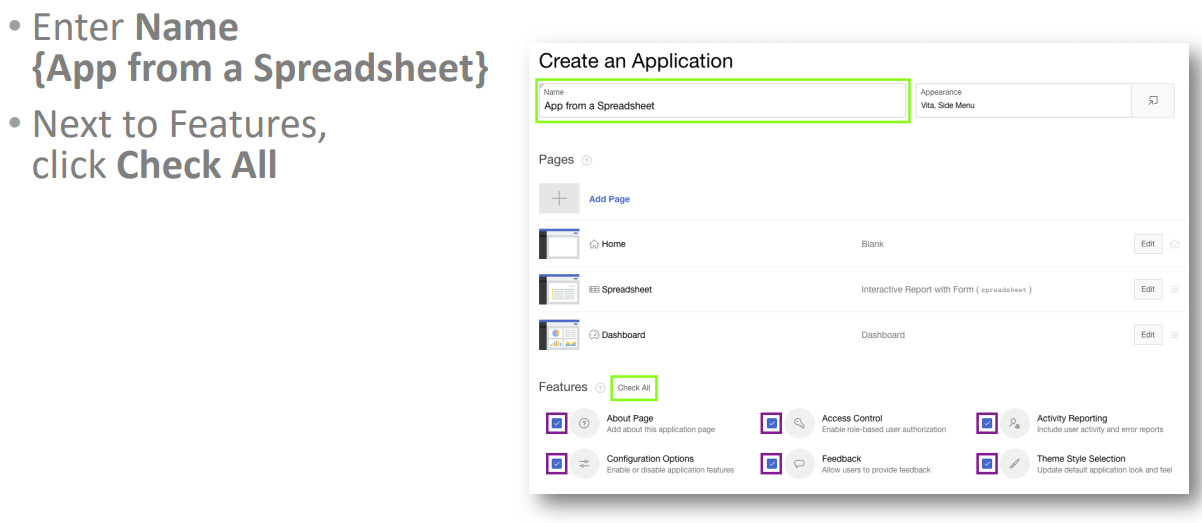
\includegraphics[scale=0.4]{figures/9.PNG}
    \caption{\textit{Naming the App.}}
        \end{center}
\label{gambar}
\end{figure}

\begin{figure}
\item[17] Load Data Sukses , klik Continue to Create Aplication.

    \begin{center}
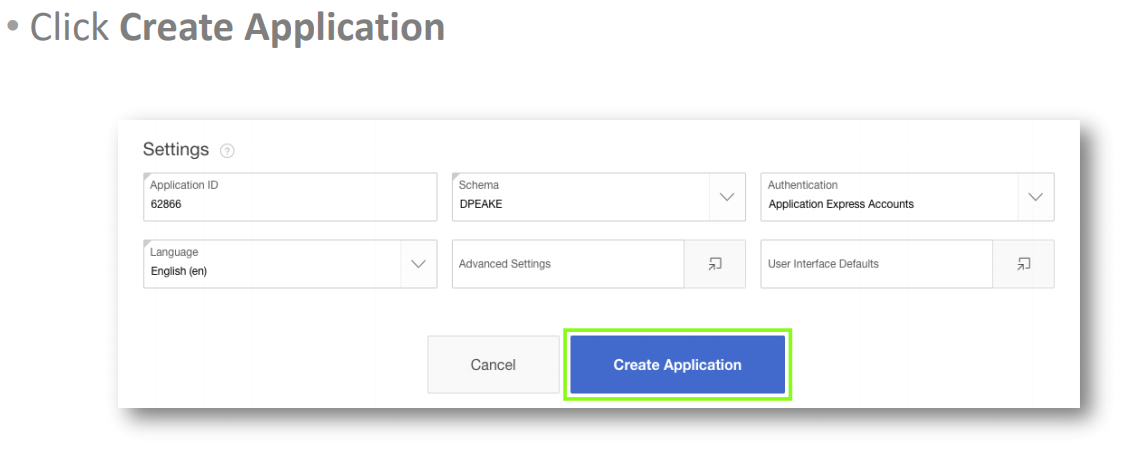
\includegraphics[scale=0.4]{figures/10.PNG}
    \caption{\textit{Create Application}}
        \end{center}
\label{gambar}
\end{figure}

\begin{figure}
\item[18]aplikasi baru anda akan ditampilkan di Page Designer

        -klik Run Application

    \begin{center}
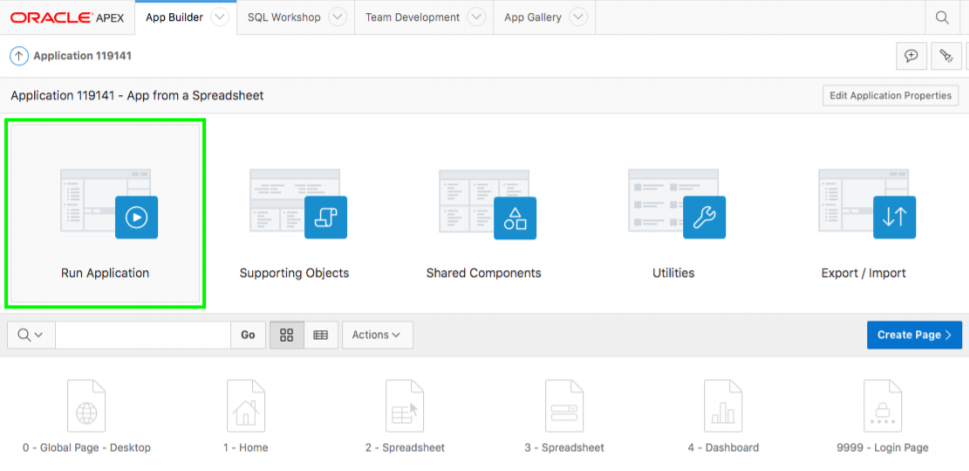
\includegraphics[scale=0.4]{figures/gambar2-8.PNG}
    \caption{\textit{Run Aplication.}}
        \end{center}
\label{gambar}
\end{figure}


\begin{figure}
\item[19]Masukkan kredensial pengguna anda, lalu jalankan aplikasi baru anda .

    \begin{center}
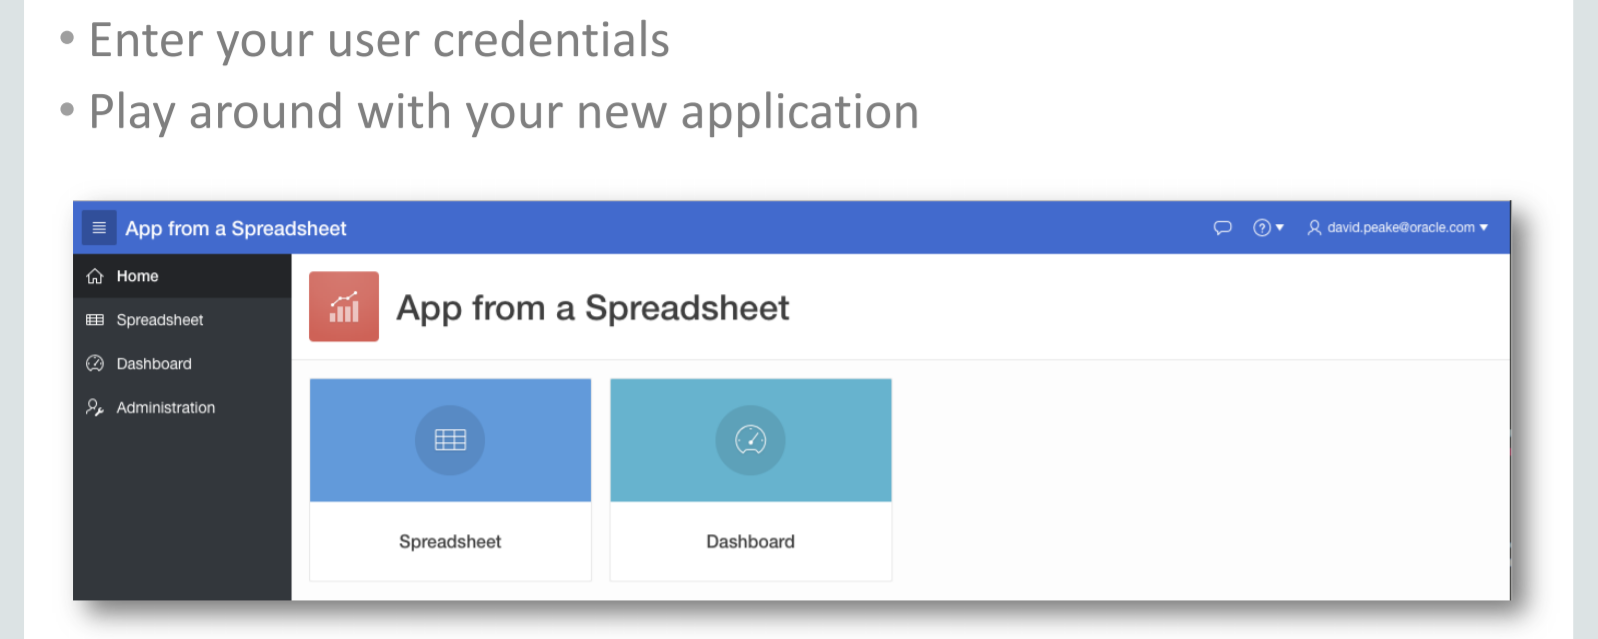
\includegraphics[scale=0.4]{figures/gambar2-9.PNG}
    \caption{\textit{Runtime App.}}
        \end{center}
\label{gambar}
\end{figure}



\end{enumerate}
